\documentclass[12pt, a4paper]{article}

\usepackage[top=2cm, bottom=2cm, left=2cm, right=2cm]{geometry}

%math packages
\usepackage{amssymb}
\usepackage{amsthm}
\usepackage{amscd}
\usepackage{amsmath}
\usepackage{enumitem}  %enumeration

\usepackage{multicol, fullpage}

\usepackage{esint} %Lines up double+ integrals
\usepackage[usenames,dvipsnames]{xcolor} % allows you to use color names, call this BEFORE you call TikZ
\usepackage{tikz, tikz-3dplot, pgfplots}
\usepackage{tkz-graph}
\usepackage{tensor}

%images
\usepackage{graphicx}
\usepackage{caption}
\usepackage{subcaption}

%\cancelto{thing cancelled to}{thing being cancelled}
\usepackage{cancel}
\usepackage{wrapfig}

% compresses items in "itemize"
\setlist{nolistsep}

%page margin package
%\usepackage[margin = 0.75 in]{geometry}

\usetikzlibrary{hobby}
\pgfplotsset{compat=1.8}


\usetikzlibrary{calc}


%\setlength{\evensidemargin}{1in}
%\addtolength{\evensidemargin}{-1in}
%\setlength{\oddsidemargin}{1.5in}
%\addtolength{\oddsidemargin}{-1.5in}
%\setlength{\topmargin}{1in}
%\addtolength{\topmargin}{-1.5in}

%\setlength{\textwidth}{16cm}
%\setlength{\textheight}{23cm}


\theoremstyle{plain}
\newtheorem{theorem}{Theorem}[section]
\newtheorem{lemma}{Lemma}
\newtheorem{proposition}{Proposition}
\newtheorem*{corollary}{Corollary}


\theoremstyle{definition}
\newtheorem{definition}{Definition}[section]
\newtheorem{notation}{Notation}
\newtheorem{question}{Question}
\newtheorem{conjecture}{Conjecture}[section]
\newtheorem{solution}{Solution}[section]
\newtheorem{example}{Example}[section]
\newtheorem{counter}{Counter Example}[section]


\theoremstyle{remark}
\newtheorem*{rem}{Remark}
\newtheorem*{note}{Note}


\def\proof{\noindent {\it Proof.} \hskip 0.1in}
\def\qed{\rightline{$\blacklozenge$}}

\newcommand{\RR}{\mathbb{R}}
\newcommand{\QQ}{\mathbb{Q}}
\newcommand{\NN}{\mathbb{N}}
\newcommand{\ZZ}{\mathbb{Z}}
\newcommand{\CC}{\mathbb{C}}
\newcommand{\II}{\mathbb{I}}

%
\begin{document}
%
%title and author details
\title{Cardiovascular Flow in Cylindrical Domain}
\author{Sean Kearns, Victor Ruiz\\
University of Colorado at Boulder\\
MATH5470}
\maketitle
\begin{abstract}
\noindent This project will briefly introduce the study of cardiovascular fluids, and discuss current analytical and numerical solutions. The Hagen-Poiseulle profile will be discussed as an example of the difficulties in constructing analytical solutions to hemodynamical problems. Also, the Arbitrary Lagrangian-Eulerian numerical technique will be presented to demonstrate the value of numerical solutions to PDEs.
\end{abstract}






\section{Analytical Problem Formulation}


\textbf{Variables}
\begin{align*}
u = u(y,z) &\equiv \; \text{Blood velocity} \\
p = p(y,z) &\equiv \; \text{Blood pressure} \\
\rho &\equiv \; \text{Blood density} \\
\mu &\equiv \; \text{Blood viscocity} \\
a &\equiv \; \text{radius} \\
\end{align*}

$\vspace{.05in}$

\textbf{Assumptions}
\begin{itemize}
\item Incompressible flow: No divergence
\item Laminar flow: No turbulence 
\item Newtonian flow: Viscous stresses proportional to the rates of change of the fluid's velocity vector
\item No-slip condition: Fluid has zero velocity relative to a solid boundary (viscous fluid)
\item Horizontal tube: No gravity affecting the system
\item Symmetric flow: $u$ becomes a function of radius exclusively
\item Steady-state flow: Properties of the fluid do not change with time %(true since functions of time aren't considered)
\end{itemize}

\newpage

Here are the incompressible Navier-Stokes equations for blood flow in 3 dimensions
\begin{align}
\frac{\partial u}{\partial t} + u \frac{\partial u}{\partial x} + v \frac{\partial u}{\partial y} + w \frac{\partial u}{\partial z} = -\frac{1}{\rho} \frac{\partial p}{\partial x} + \frac{\mu}{\rho} \Delta u\\
\frac{\partial v}{\partial t} + u \frac{\partial v}{\partial x} + v \frac{\partial v}{\partial y} + w \frac{\partial v}{\partial z} = -\frac{1}{\rho} \frac{\partial p}{\partial y} + \frac{\mu}{\rho} \Delta v\\
\frac{\partial w}{\partial t} + u \frac{\partial w}{\partial x} + v \frac{\partial w}{\partial y} + w \frac{\partial w}{\partial z} = -\frac{1}{\rho} \frac{\partial p}{\partial z} + \frac{\mu}{\rho} \Delta w
\end{align}
over the circular cylindrical domain as expressed in the figure below from Y.C. Fung $\cite{Father}$.

\begin{figure}[ht!]
\centering
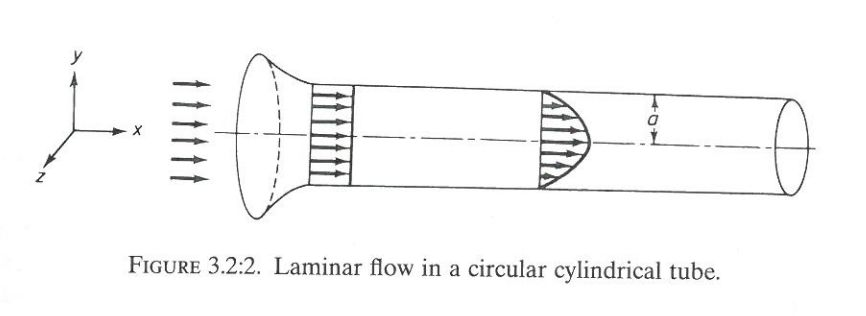
\includegraphics[width=100mm]{cardiovasculardomain.jpg}
\end{figure}
The parabolic velocity profile of the Hagen-Poiseulle flow $u(r)$ as well as the flow rate $Q$ through a cross-section of the cylindrical domain above are presented below:
\begin{align}
u(r)  &= - \frac{1}{4\mu} \frac{\partial p}{\partial x} \left[  a^2-r^2        \right] \\
Q     &=- \frac{\pi a^4}{8\mu} \frac{\partial p}{\partial x} 
\end{align}
given the boundary conditions $u=0$ at $r=a$, and $\partial u/\partial r  = 0$ at $r=0$.

\section{Numerical Method}


The Arbitrary Lagrangian-Eulerian method is commonly used for computational blood flow with respect to  tube and bifurcation models. This particular method is a combination of the Lagrangian and Eulerian descriptions of motion, where their respective advantages are combined while minimizing drawbacks $\cite{carotid}$. 


\textbf{Lagrangian:}
Each individual node of the computational mesh follows the associated material particle motion, which allows for an easy tracking of free surfaces and interfaces between materials. The method is unable to accurately follow large distortions of the computational domain $\cite{ALE}$. 

\textbf{Eulerian:}
The computational mesh is fixed and the continuum moves with respect to the grid. The method is capable of handling large distortions easily, but generally at the expense of precise interface definition and resolution of flow details $\cite{ALE}$.

\textbf{Arbitrary Lagrangian-Eulerian Method:}
Nodes of the computational mesh may be moved with the continuum in a normal Lagrangian fashion, or be held in a fixed Eulerian manner. The ability to accommodate significant distortions of the computational mesh, while preserving the clear delineation of interfaces typical of a purely lagrangian approach allows for the modeling of an elastic boundary that does not depend solely on the fluid motion $\cite{ALE}$.

Using FEMLAB (numerical solutions), and ALE (computational mesh construction--boundary/domain) to model the domain given 893 CT scan images of an arbitrary patient's carotid artery, CAD models were generated for both the vessel itself (Figure 2), as well as with altered boundary conditions introducing simulations for vasoconstriction and vasodilation (Figure 3). 

\textbf{Assumptions}

\begin{itemize}
\item Incompressible flow: No divergence
\item Newtonian flow: Viscous stresses proportional to the rates of change of the fluid's velocity vector
\item Axisymmetric flow: Cylindrical symmetry
\item Blood properties:
\begin{itemize}
\item $\mu = 0.005$ N$\cdot$s/m$^2$
\item $\rho = 1060$ kg/m$^3$
\end{itemize}
\item Arterial wall properties:
\begin{figure}[ht!]
\centering
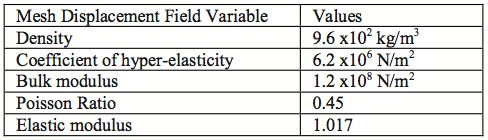
\includegraphics[width=100mm]{arterywallproperties.jpg}
\end{figure}
\end{itemize}
\begin{wrapfigure}[13]{l}{0.5\textwidth}
    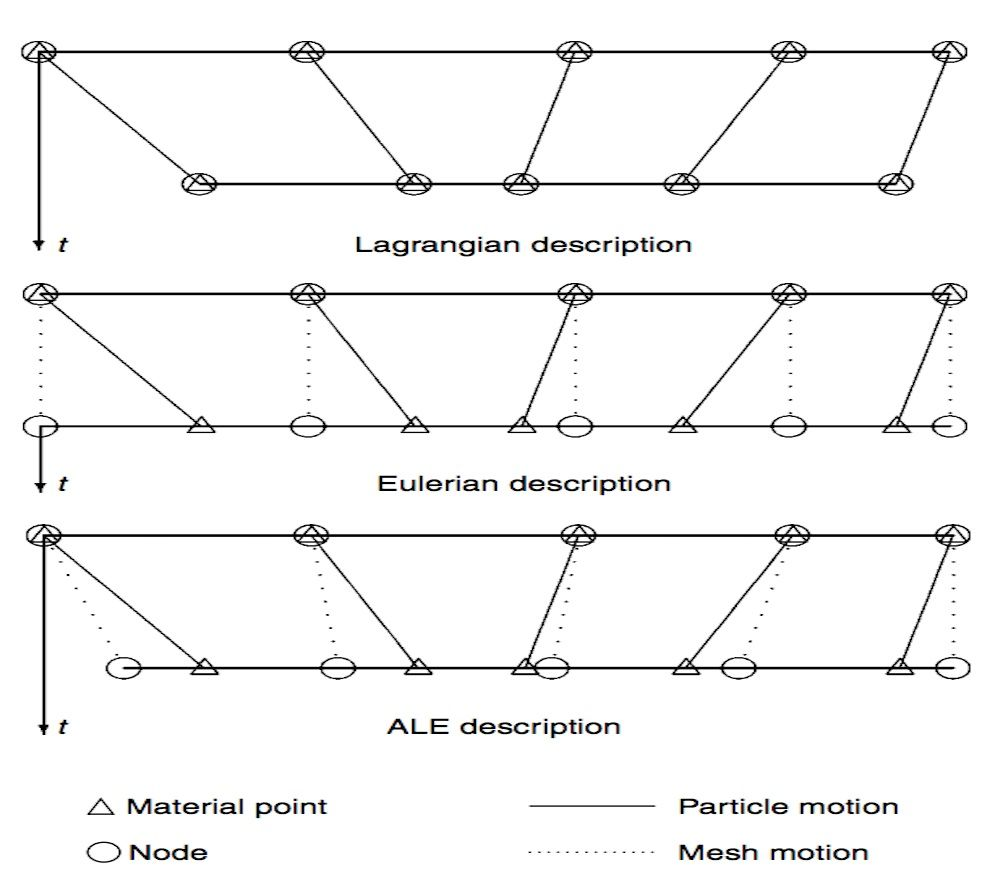
\includegraphics[width=0.53\textwidth]{lagrangianeuleriann.jpg}
  \caption{1D example of Lagrangian, Eulerian and
ALE mesh and particle motion $\cite{ALE}$.}
\end{wrapfigure}

$\vspace{.18in}$

\noindent The 2D incompressible Navier-Stokes equations below were used for cardiovascular flow $\cite{ALE}$,$\cite{carotid}$. Note that time is considered in this example. 
\begin{align*}
\rho \left(      \frac{\partial u}{\partial t} + u\frac{\partial u}{\partial x} + v\frac{\partial u}{\partial y}         \right) = -\frac{\partial p}{\partial x} + \mu\Delta u \\
\rho \left(      \frac{\partial v}{\partial t} + u\frac{\partial v}{\partial x} + v\frac{\partial v}{\partial y}         \right) = -\frac{\partial p}{\partial x} + \mu \Delta v 
\end{align*}

\noindent Also, Figure 1 is a visual representation of the comparison between the Lagrangian, Eulerian, and ALE descriptions of motion for particles within the domain, as well as the domain boundary itself.  

%\begin{align*}
%\rho \left(      \frac{\partial u(x,t)}{\partial t} + u(x,t)\frac{\partial u(x,t)}{\partial x} + v(y,t)\frac{\partial u(x,t)}{\partial y}         \right) = -\frac{\partial p}{\partial x} + \mu \left(  \frac{\partial^2 u(x,t)}{\partial x^2} +\frac{\partial^2 u(x,t)}{\partial y^2}    \right) \\
%\rho \left(      \frac{\partial v(y,t)}{\partial t} + u(x,t)\frac{\partial v(y,t)}{\partial x} + v(y,t)\frac{\partial v(y,t)}{\partial y}         \right) = -\frac{\partial p}{\partial x} + \mu \left(  \frac{\partial^2 v(y,t)}{\partial x^2} +\frac{\partial^2 v(y,t)}{\partial y^2}    \right) 
%\end{align*}

\newpage

\begin{figure}[ht!]
\centering
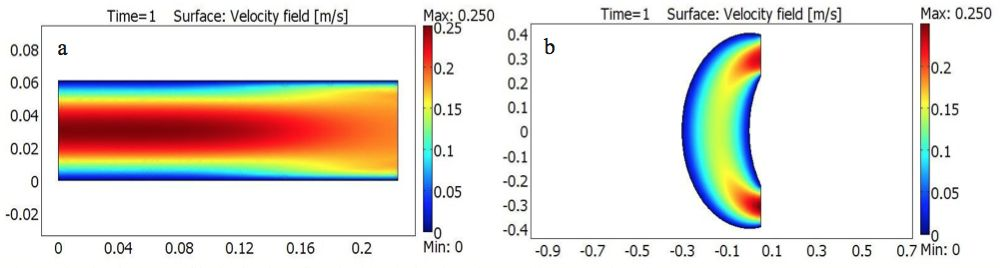
\includegraphics[width=150mm]{carotidartery.jpg}
\caption{Patient X carotid artery blood velocity profile for laminar flow in (a) tubular domain and (b) curved domain $\cite{carotid}$.}
\end{figure}
\begin{figure}[ht!]
\centering
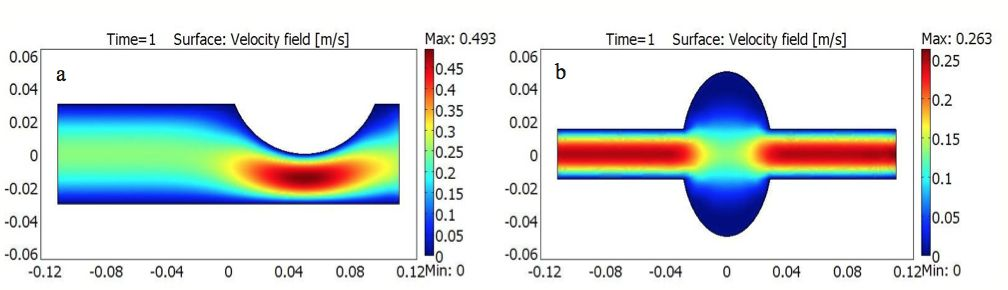
\includegraphics[width=150mm]{vasoconstriction.jpg}
\caption{Blood velocity field with irregular flow pattern resulting from (a) vasoconstriction and (b) vasodilation $\cite{carotid}$.}
\end{figure}


It is important to note that the complexity of these boundary value problems typically pose difficulties in determining the convergence of solutions $\cite{carotid}$.


 \begin{thebibliography}{1}
 \bibitem{history} Alfio Quarteroni, {\em Modeling the Cardiovascular System--A Mathematical Adventure: Part I.} 2001: SIAM News 34.5 (2001): 1-3.

  \bibitem{n-seq} C Y Wang, {\em Exact solutions of the unsteady Navier-Stokes equations.} 1989: American Society of Mechanical Engineers.

   \bibitem{ALE} J. Donea et al. {\em Arbitrary Lagrangian-Eulerian Methods.} 2004: Encyclopedia of computational mechanics.

  \bibitem{carotid}  Jhalique Jane R. Fojas, Rizalinda L. De Leon, {\em Carotid Artery Modeling Using the Navier-Stokes Equations for an Incompressible, Newtonian and Axisymmetric Flow.} 2013: Asia-Pacific Chemical, Biological $\&$ Environmental Engineering Society.

  \bibitem{Biofluid} Perumal Nithiarasu {\em Biofluid Dynamics.} 2008: Swansea University, United Kingdom.

  \bibitem{Father} Yuan-cheng Fung. {\em Biomechanics: circulation}. 1997: Springer.
  \end{thebibliography}













\end{document}